%!TEX root =mpip.tex
\section{the Design}
\label{sec:design}
Based on Linux kernel $3.12$, the implementation is mainly at the network layer and targets to IP protocol. To make the implementation transparent to users and other layers, we try to keep all kernel modifications independent from other modules. To keep the simplicity of IP protocol, we keep the connectionless feature of IP protocol while maintaining some feedback information of different paths. As will be shown later, we achieve this goal by simply keeping track of several tables. This can make sure that we don't add excessive overhead to the system.

As a fundamental problem, NAT devices are commonly used in the current Internet. For a single connection, multiple NAT devices can exist on the path. With the existence of NAT devices, many IP addresses are exposed to the Internet as a combination of IP address and port number. So in the following sections, when referring the address of a node, we will use the combination of IP address and port number.


%\subsection{MPIP Working Modes}
%As we can see, assume there are $M$ and $N$ networking interfaces on each end, there will be $M*N$ available paths totally between the two nodes. Among all the available paths, we can have different modes to make use of them. Generally, there are two modes of MPIP.
%
%\begin{enumerate}
%\item Parallel mode. In parallel mode, all available interfaces will send out packets that are assigned to them. The number of packets that are assigned to them is calculated according to their relative capability. In parallel mode, all available interfaces will be used to transmit packets. There can be two scenarios. If the packet passed down is large enough (larger than some threshold value), the packet will be to be sent out through more than one interface. In this case, one unique token for all fragments, fragmentation offset, and the information about the main IP address will be contained in the options data in the IP header. The receiver will merge all the data together into the packet from the main IP address and pass it to the upper layer. If one of the fragments lost during the transmission, the whole packet will fail after some expiration time. The data size that is assigned to each path is calculated through their capability. If the packet passed down doesn't need any fragmentation because it is a small one, then we need to choose one path to send out the packet. In this case, random number is used to choose the final path according to their capability.
%
%\item Backup mode. In back-up mode, there is only one working interface. Other interfaces will be the backup interfaces which means that the backup interface will take over the connection when the working interface isn't available. In backup mode, that is only the main interface that is used to transmit packets that are passed down from upper layer. If the current working main interface isn't the one when the connection was initiated, MPIP module needs to add the original interface information into the options field of IP header to tell the receiver the destination of this packet. If the current working main interface is the same as the initial one, nothing is going to change. The receiver won't do any additional process for the packet once it receives it, just passes it to the upper layer.
%\end{enumerate}
%
%In both parallel mode and backup mode, there is a main interface which is used to notate the connection. In parallel mode, one main interface is chosen when the application starts the connection. In backup mode, the working interface is the main interface. In both modes, when the main interface isn't available at any time, other interfaces will take over seamless and act as the main interface without being known by upper layers because this main interface is maintained at the transport layer. With this mechanism, all connection won't be re-established after interface switching.

\subsection{IP Layer Control Communication}
In TCP protocol, the ACK packet is mainly used as the feedback information from the receiver. Then the sender is able to know the real time status of the transmission. But IP protocol doesn't have this built-in feedback loop because it is a connectionless protocol. To maintain multiple paths at IP layer, we need to add control communication functionality like the ACK packet in TCP. Instead of constructing new control packets between connection ends, we use piggyback technology to implement the feedback message in IP layer. This can avoid excessive control packets and reduce overhead of MPIP.

For each MPIP enabled packet that goes out of the system, we add an additional control message(CM) data block at the end of user data.
%The size of the CM block is $25$ bytes which is the communication overhead of MPIP, this is trivial comparing to the benefit brought by MPIP.
Sometimes the size of the packet will exceeds MTU after attaching the data block. In this case, we reduce the amount of user data from transportation layer to fit the CM block, e.g, we decrease the MSS value for TCP connection.

%\begin{figure}
%\centering
%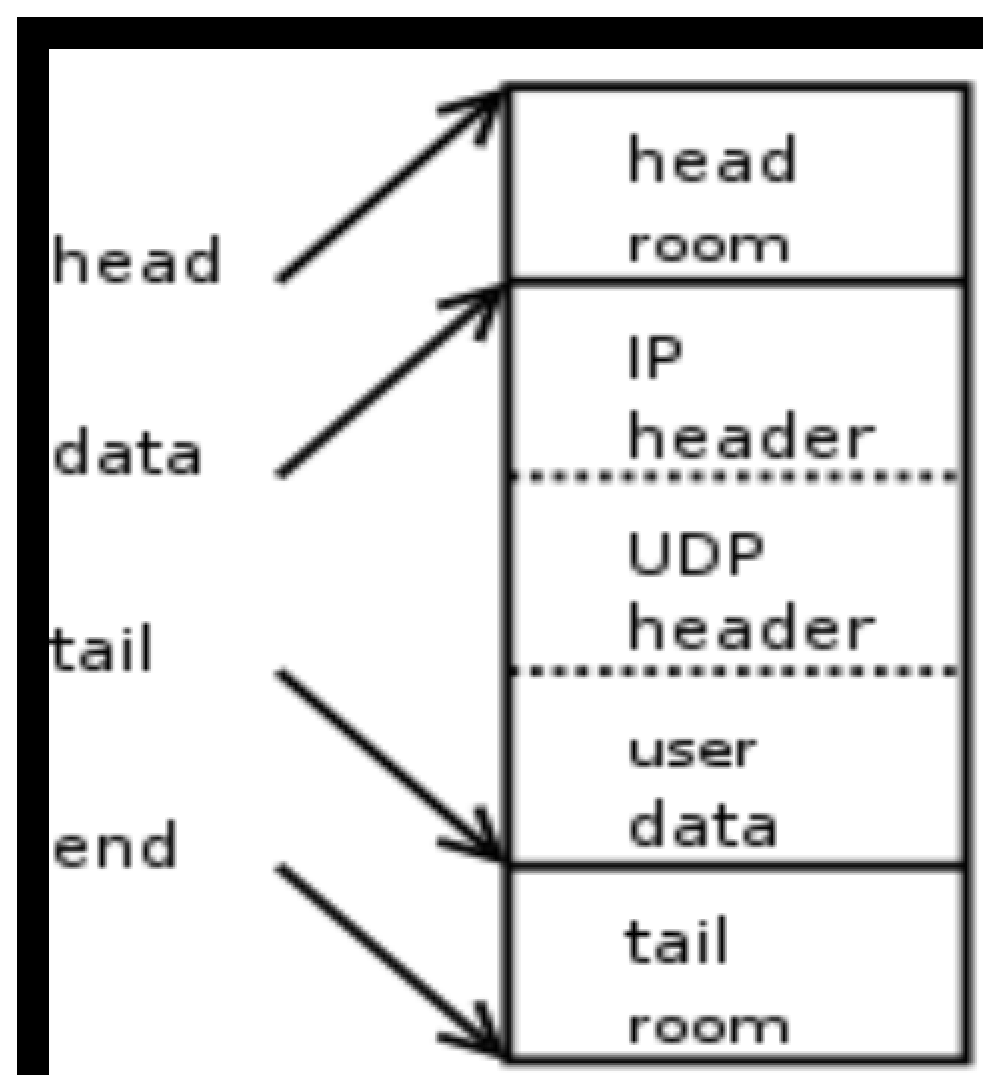
\includegraphics[width=0.8\linewidth]{fig/cm.eps}
%\caption{CM data block}
%\label{fig.cm}
%\end{figure}


The content in the control message is shown in Table~\ref{tb.cm}.

\begin{table}
\caption{\label{tb.cm}Control Message Structure}
\centering
\begin{tabular}{|c|}
\hline
Control Message \\
\hline
\emph{Node ID,} \\
\emph{Session ID,} \\
\emph{Path ID,} \\
\emph{Feedback Path ID,} \\
\emph{Packet Timestamp,} \\
\emph{Path Delay}\\
\emph{Local Address List}\\
\emph{CM Flags}\\
\emph{Checksum}\\
\hline
\end{tabular}
\end{table}

\emph{Node ID} is the globally unique identification of one node. The combination of IP address and port number is not a qualified candidate because during connection switching, IP address can change on a specific NIC. To have a static node ID, we choose the MAC address of any one NIC on the node to be the unique ID.
The value of node ID is initiated when the system starts and keep it unchanged until the system exits. Every time the node sends out a packet, it fills the field of \emph{node ID} with this value into the control message.

\emph{Local Address List} carries all local IP addresses. This list will be used to construct new MPIP paths.

\emph{CM Flags} notates the functionality of the packet. With different value of \emph{CM Flags}, different action will be taken when the packet is received.

\emph{Checksum} is used to verify the validation of the CM data block. This value is assigned by simply adding up the value of all other field in the CM data block. This will be recalculated when received to judge whether a CM data block is attached in this packet. The packet will be treated as a normal packet if the checksum verification doesn't get through.

Other fields of the CM block will be explained in following sections.

\subsection{MPIP availability handshake}
\label{sec:handshake}

As a new feature in Linux, MPIP needs to be backward compatible. For one specific connection, before enabling MPIP at both end, the two sides need to synchronize with each other to make sure both are MPIP enabled. Locally, every node maintains Table~\ref{tb.me} to identify the availability of MPIP for its opposite nodes. Before the handshake finishes, all communication on the connection is normal traffic without MPIP enabled.

\begin{table}[htbp]
\caption{\label{tb.me}MPIP availability}
\centering
\begin{tabular}{|c|c|c|c|}
\hline
IP 		& Port 	 & MPIP 		   & Query\\
Address & Number & Availability & Count\\
\hline
${IP}_{1}$ & ${P}_{1}$ & True  & $2$ \\
\hline
${IP}_{2}$ & ${P}_{2}$ & False & $5$ \\
\hline
\end{tabular}
\end{table}


When a node sends out a packet, it checks locally whether the target node is MPIP enabled in Table~\ref{tb.me}. If not, besides sending out the original packet, the system copies the current packet and inserts the CM block into the copied packet with \emph{CM Flags} of $Flags\_Enable$. This value is used for MPIP query. When this packet is received by a MPIP enabled node, the receiver adds the sender's IP address and port number into Table~\ref{tb.me} with value of $True$, then sends back the confirmation to the sender with \emph{CM Flags} of $Flags\_Enabled$ at a proper time. For TCP and non-TCP connection, we send out the confirmation packet at different times. For any protocol rather than TCP, we populate a new packet, fill all header fields with the correct information, and attach the CM block at the end, then send back to the sender right away. But for TCP, we add the confirmation request into a waiting list, and piggyback the confirmation when next TCP message is sent out to that specific node. There are two reasons to have this different process.

\begin{enumerate}
\item For protocols rather than TCP, like UDP, because they don't have built-in feedback loop, which means that all traffic can be one direction. In this scenario, we can't wait until there are packets available to piggyback the confirmation.

\item For TCP protocol, we don't simply populate a new TCP packet and send back because the sequence numbers of each direction are way different. Through our experiments, some NAT devices will refuse to transfer this packet if the sequence number messes up for the same TCP connection. To solve this problem, we add the request into a waiting list. When there are TCP packets available to send , we make a copy of the packet and attach the CM block with \emph{CM Flags} of $Flags\_Enabled$ to send out. In this case, there will be two consecutive TCP packets with the same sequence number. The NAT devices will simply consider them as retransmissions instead of dropping them.
\end{enumerate}

For both the MPIP query packet and MPIP confirmation packet, we populate new packets based on the original packets by making copies. All copied packets won't be passed to higher layers, they are generated at network layer and stop there too, they don't mean anything to higher layers. The network layer drops all MPIP packets with \emph{CM Flags} of $Flags\_Enable$ and $Flags\_Enabled$ after processing them. The MPIP handshake process is shown in Figure~\ref{fig.handshake}.

\begin{figure}
\centering
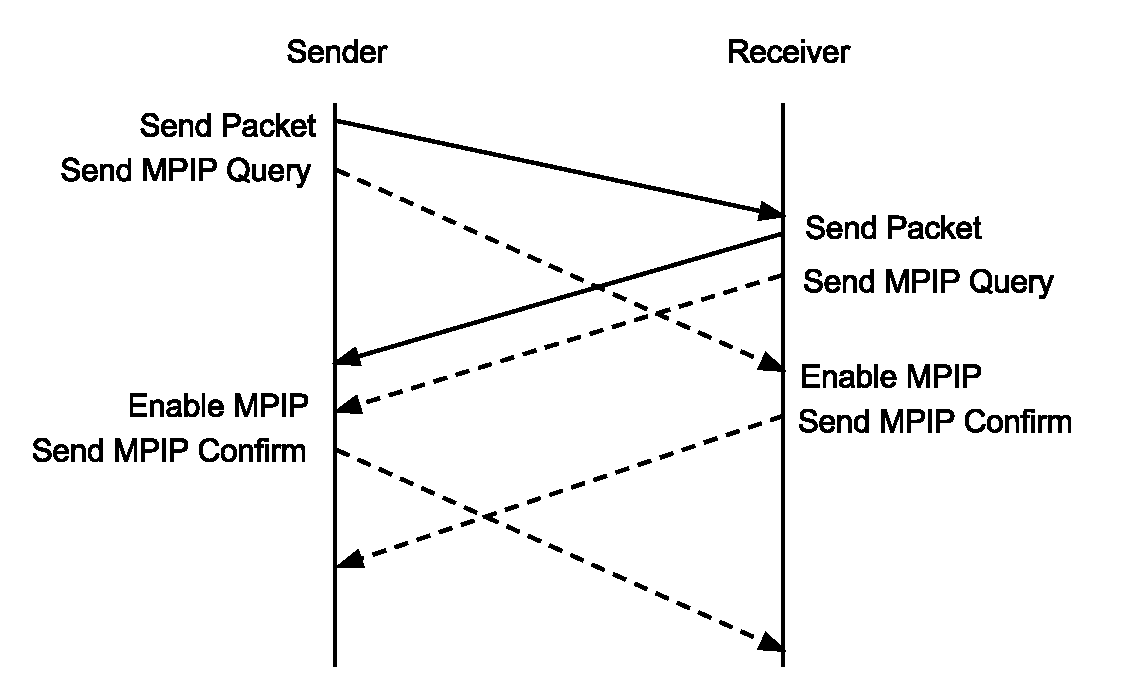
\includegraphics[width=0.8\linewidth]{fig/handshake.eps}
\caption{MPIP Handshake}
\label{fig.handshake}
\end{figure}

With the handshake flow above, the smallest number of query packet that will be sent for the whole process is only one. But sometimes because of packet loss or synchronization issues, there can be multiple query packet sent out at both ends as shown in Figure~\ref{fig.handshake}. This is not a problem because the design of the system allows receiving more than one query packet and confirmation packet. But on the other hand, for nodes that don't support MPIP, we can't send out query messages forever. In Table~\ref{tb.me}, the column \emph{Query Count} maintains the number of query messages that have been sent out to relative IP addresses. If the number is larger than a threshold value, it assumes that IP address doesn't support MPIP. Considering that packet loss is rare event in Internet nowadays, we set this value to $5$ in our system, this is more than enough to make sure a MPIP enabled node can receive and reply this message with successful transmissions. In a connection with only one-way traffic, if the receiver is MPIP enabled while the sender isn't, then no query packet will be sent out at all.

Generally, for MPIP enabled nodes, they may have more than one IP address. In this situation, multiple synchronization messages will be transmitted for the same node.


\subsection{Path Management}
\label{sec:path}

Given $M$ and $N$ interfaces at each end of one connection, there are totally $M*N$ possible paths on the connection. In our system, we maintain all available paths through Table~\ref{tb.pi}.

\begin{table*}
\small
\caption{\label{tb.pi}Path information}
\centering
\begin{tabular}{|c|c|c|c|c|c|c|c|c|c|c|c|}
\hline
Node &  Path & Session & Src &   Src & Dest & Dest &   Minimum       & Real-Time      & Real-Time      & Maximum       & Path   \\
 ID  &   ID  & ID & IP  &  Port &  IP  & Port &  Network Delay  & Network Delay  & Queuing Delay  & Queuing Delay & Weight \\
\hline
$ID$&${PID}_{11}$&${SID}_{1}$&${SIP}_{1}$&${SP}_{1}$&${DIP}_{1}$&${DP}_{1}$&${D_{min}}_{11}$&$D_{11}$&${Q}_{11}$&${{Q}_{max}}_{11}$&$W_{11}$\\
\hline
$ID$&${PID}_{12}$&${SID}_{1}$&${SIP}_{1}$&${SP}_{1}$&${DIP}_{1}$&${DP}_{2}$&${D_{min}}_{12}$&$D_{12}$&${Q}_{12}$&${{Q}_{max}}_{12}$&$W_{12}$\\
\hline
$ID$&${PID}_{21}$&${SID}_{2}$&${SIP}_{1}$&${SP}_{2}$&${DIP}_{1}$&${DP}_{1}$&${D_{min}}_{21}$&$D_{21}$&${Q}_{21}$&${{Q}_{max}}_{21}$&$W_{21}$\\
\hline
$ID$&${PID}_{22}$&${SID}_{2}$&${SIP}_{1}$&${SP}_{2}$&${DIP}_{1}$&${DP}_{2}$&${D_{min}}_{22}$&$D_{22}$&${Q}_{22}$&${{Q}_{max}}_{22}$&$W_{12}$\\
\hline
\end{tabular}
\end{table*}

Node ID is used to identify the other end of connections. Path ID is used to identify one path. It is a locally unique Arab numbers starting from $1$. This value is generated only when adding new paths into Table~\ref{tb.pi}.

Because of NAT mapping, the same node can have different IP address and port number that will be seen on the other side at different time or even for different application. That's why column \emph{Session ID} needs to be added into Table~\ref{tb.pi}. When sending out one packet, the final path will only be chosen from the ones that have the correct session id. The detail of session is explained in Section~\ref{sec:session}. Here we just consider a session is the synonym of one connection. As the names show, source IP, source port, destination IP and destination port show the address information of the path.

%The IP addresses here are the addresses that are seen by the node that maintain the instance of Table~\ref{tb.pi}. This value might be different from local IP addresses because of NAT mapping.

One instance of Table~\ref{tb.pi} is maintained at each side. Initially, Table~\ref{tb.pi} is empty. Every time one new combination of IP address and port number is flagged as MPIP enabled in Table~\ref{tb.me}, it adds new paths to the table with every available local IP address as the source IP address, and the value of Node ID is extracted from Table~\ref{tb.wi} which is maintained to conveniently map node ID with IP address and port number.

%Table~\ref{tb.wi} contains all working IP addresses and port number of one specific node ID. When paths in Table~\ref{tb.pi} are obsolete and need to be removed, relative entries in Table~\ref{tb.wi} will also be removed.

\begin{table}[htbp]
\caption{\label{tb.wi}Node ID vs IP address and Port}
\centering
\begin{tabular}{|c|c|c|}
\hline
 Node ID  & IP Address & Port Number\\
\hline
${ID}_{1}$&${IP}_{11}$&${P}_{11}$ \\
\hline
${ID}_{1}$&${IP}_{12}$&${P}_{12}$ \\
\hline
${ID}_{2}$&${IP}_{21}$&${P}_{21}$ \\
\hline
${ID}_{2}$&${IP}_{22}$&${P}_{22}$ \\
\hline
\end{tabular}
\end{table}

For multipath connections with full mesh, if both $M$ and $N$ are larger than $1$, every NIC is reused at least once. Sometimes it is not necessary to reuse them because of system overhead consideration; In this use case, we can limit the number of available paths for one session to be $l$, then only the fastest $l$ paths will be used, other paths will be abandoned.

\subsection{Feedback Loop}
\label{sec:feedback}

Packet loss and delay are the most important two characters of one path. Given that packet loss in current Internet has become rare events, we only focus on delay in our system. Furthermore, different paths can be chosen on different side, round trip delay doesn't work for MPIP. Based on this, we implement IP layer's feedback loop with one-way delay as the feedback variable.

In Table~\ref{tb.pi}, all fields referring to network delay will be filled or calculated by feedbacked one-way delay. In Table~\ref{tb.cm}, the fields \emph{Path ID} and \emph{Packet Timestamp} are used to measure network delay. When node $A$ sends out a packet, it chooses a path from Table~\ref{tb.pi}, fill the field \emph{Path ID} with the chosen path ID, and fill the filed \emph{Packet Timestamp} with local system time $T_1$ in the CM block. After node $B$ receives this packet, it extracts node ID, path ID and timestamp from the CM block. The node ID and path ID are directly used to identify records in Table~\ref{tb.ps}, and node $B$ uses $T_2-T_1$ as the one-way delay from node $A$ to node $B$ where $T_2$ is the local system time when receiving the packet. Node $B$ checks whether the path that identified by the node ID and path ID already exists in Table~\ref{tb.ps}, if yes, it updates the path's delay with $T_2-T_1$, otherwise, it adds a new record into Table~\ref{tb.ps}.

\begin{table}[htbp]
\caption{\label{tb.ps}Path Feedback information}
\centering
\begin{tabular}{|c|c|c|c|c|c|}
\hline
 Node   & Path    & Path      & Feedback           \\
  ID    &  ID     & Delay     & Time               \\
\hline
${ID}_{11}$&${PID}_{11}$&${D}_{11}$&${T}_{11}$   \\
\hline
${ID}_{12}$&${PID}_{12}$&${D}_{12}$&${T}_{12}$   \\
\hline
${ID}_{21}$&${PID}_{21}$&${D}_{21}$&${T}_{21}$   \\
\hline
${ID}_{22}$&${PID}_{22}$&${D}_{22}$&${T}_{22}$   \\
\hline
\end{tabular}
\end{table}

In practice, the value of path delay calculated here isn't the real delay value because of time difference between node $A$ and node $B$ as shown in \ref{sec:clock}, it can even be negative. But as we will see later, time difference between $A$ and $B$ doesn't have any influence on our algorithm.

When node $B$ needs to send packet back to node $A$, it chooses the record with the earliest feedback time from Table~\ref{tb.ps}, fills the field \emph{Feedback Path ID} and \emph{Path Delay} in the CM block, and updates the column \emph{Feedback Time} with local system time. When node $A$ receives this feedback packet, it extracts the path ID and path delay value, and fills the path delay value into the column \emph{Real-Time Network Delay} in Table~\ref{tb.pi}. To avoid outliers, the value of path delay is calculated by moving average algorithm.

%At meantime, the column \emph{Feedback Time} is updated with current system time. If one path hasn't received feedback information from the receiver for some threshold value of time, it means this path is literally dead, then the system considers the path to be obsolete and remove the path from Table~\ref{tb.pi}.


\subsubsection{Dynamic Addition/Removal of Paths}
\label{sec:switch}

As multipath feature enabled on a device, IP addresses of devices can be removed or added dynamically. Especially for mobile device, it can connect to different access points(WiFi hotspot/Cellular Tower) at different time, during this stage, its IP address can be changed, removed or added dynamically. Under this situation, the system supports dynamic addition and removal of paths from Table~\ref{tb.pi}.

When IP address change happens, the value of \emph{CM Flags} is set to be $Flags\_IP\_Change$ in the CM block when sending out packets. After receiving packets of this flag, the receiver knows that IP address change happened on the sender, it will remove all entries of this connection in all tables, then add the combination of IP address and port number contained in the received packet into all the tables as if that combination is MPIP enabled.
Also, the sender does the same reset for this connection. After all these resets, there is only one path left for this connection, all the other paths will be added into the system through the normal process. By doing this path reconstruction, we achieve smooth transmission during IP address changes which is transparent to higher layers.


\subsection{Periodical Heartbeat}

For protocols like TCP, during the whole lifetime of the connection, both sides are sending packets to each other at a high frequency, then at both sides, Table~\ref{tb.pi} can be updated real-time. But there are protocols that don't have this built-in feedback mechanism, like UDP. In some UDP applications, all traffic is one way, there aren't any acknowledgements, which means that the sender can't get feedback information through piggybacked messages. Under this scenario, the sender won't be able to properly add new entries into Table~\ref{tb.pi}, then multipath feature can't be applied at all.

To solve this problem, a periodical heartbeat mechanism is introduced into the design. At each side, when the node receives packets, the system checks Table~\ref{tb.ps} for the specific node, if it finds the feedback time of this path is close to a pre-set value, it makes a copy of the received packet, switches the source/destination address information, and sends back the packet with CM block attached. The path to send this heartbeat message will be chosen through the same algorithm as regular IP packet as in Section~\ref{sec:selection}. Through the heartbeat message, we effectively maintain the real-time status of each path between two nodes for connections with one-way traffic. The expiration time of heartbeat message is set to $300$ms in our system.

All heartbeat packets have a special flags value $Flags\_HB$ in the CM block. These packets will be dropped after being processed at network layer.

\subsection{Path Selection}
\label{sec:selection}

Every time one node needs to send out packets, it chooses the most suitable path from Table~\ref{tb.pi}. Depends on the requirement of throughput and responsiveness, we have different considerations to choose the target path.

\subsubsection{Delay-based Path Selection}
\label{sec:delay}
In the current Internet, there are many high delay-bandwidth product connections. These connections generally have both high delay and high bandwidth. For applications that want to achieve high throughput, we propose following mechanism to achieve the requirement.

The criterion of choosing the best path that can achieve high throughput is on the column of \emph{Path Weight}. Given certain values of this column, we don't simply choose the path that has the largest path weight which may overuse the path and starve other paths. Instead, we choose the path by random number. For one specific path $k$, the probability $P(k)$ it will be chosen is calculated in Equation~\ref{eq.choose}. By balancing the percentage of packets on each path, system fluctuation can be effectively avoided.

\be
\label{eq.choose}
P(k) = \frac{W_k}{\sum_{i=1}^{N}W_i}
\ee

From above, the path weight is the only criterion to choose the target path, so the calculation of path weight $W$ is critical to the performance of the system. Wrong decision can result in catastrophic disaster. In our prototype, by introducing delay-based solution, we calculate the value of $W$ in an incremental pattern.

For network delay, it consists of following $4$ parts.

\begin{enumerate}
\item Processing delay. Time routers take to process the packet header
\item Queuing delay. Time the packet spends in routing queues
\item Transmission delay. Time it takes to push the packet onto the link
\item Propagation delay. Time for a signal to reach its destination
\end{enumerate}

Among the four parts above, processing delay, transmission delay and propagation delay are fixed value for one path, they can be treated as constant. But queuing delay changes as the traffic load on the path changes. Figure~\ref{fig.delay} shows the trend of network delay as of the traffic on the path changes.

\begin{figure}
\centering
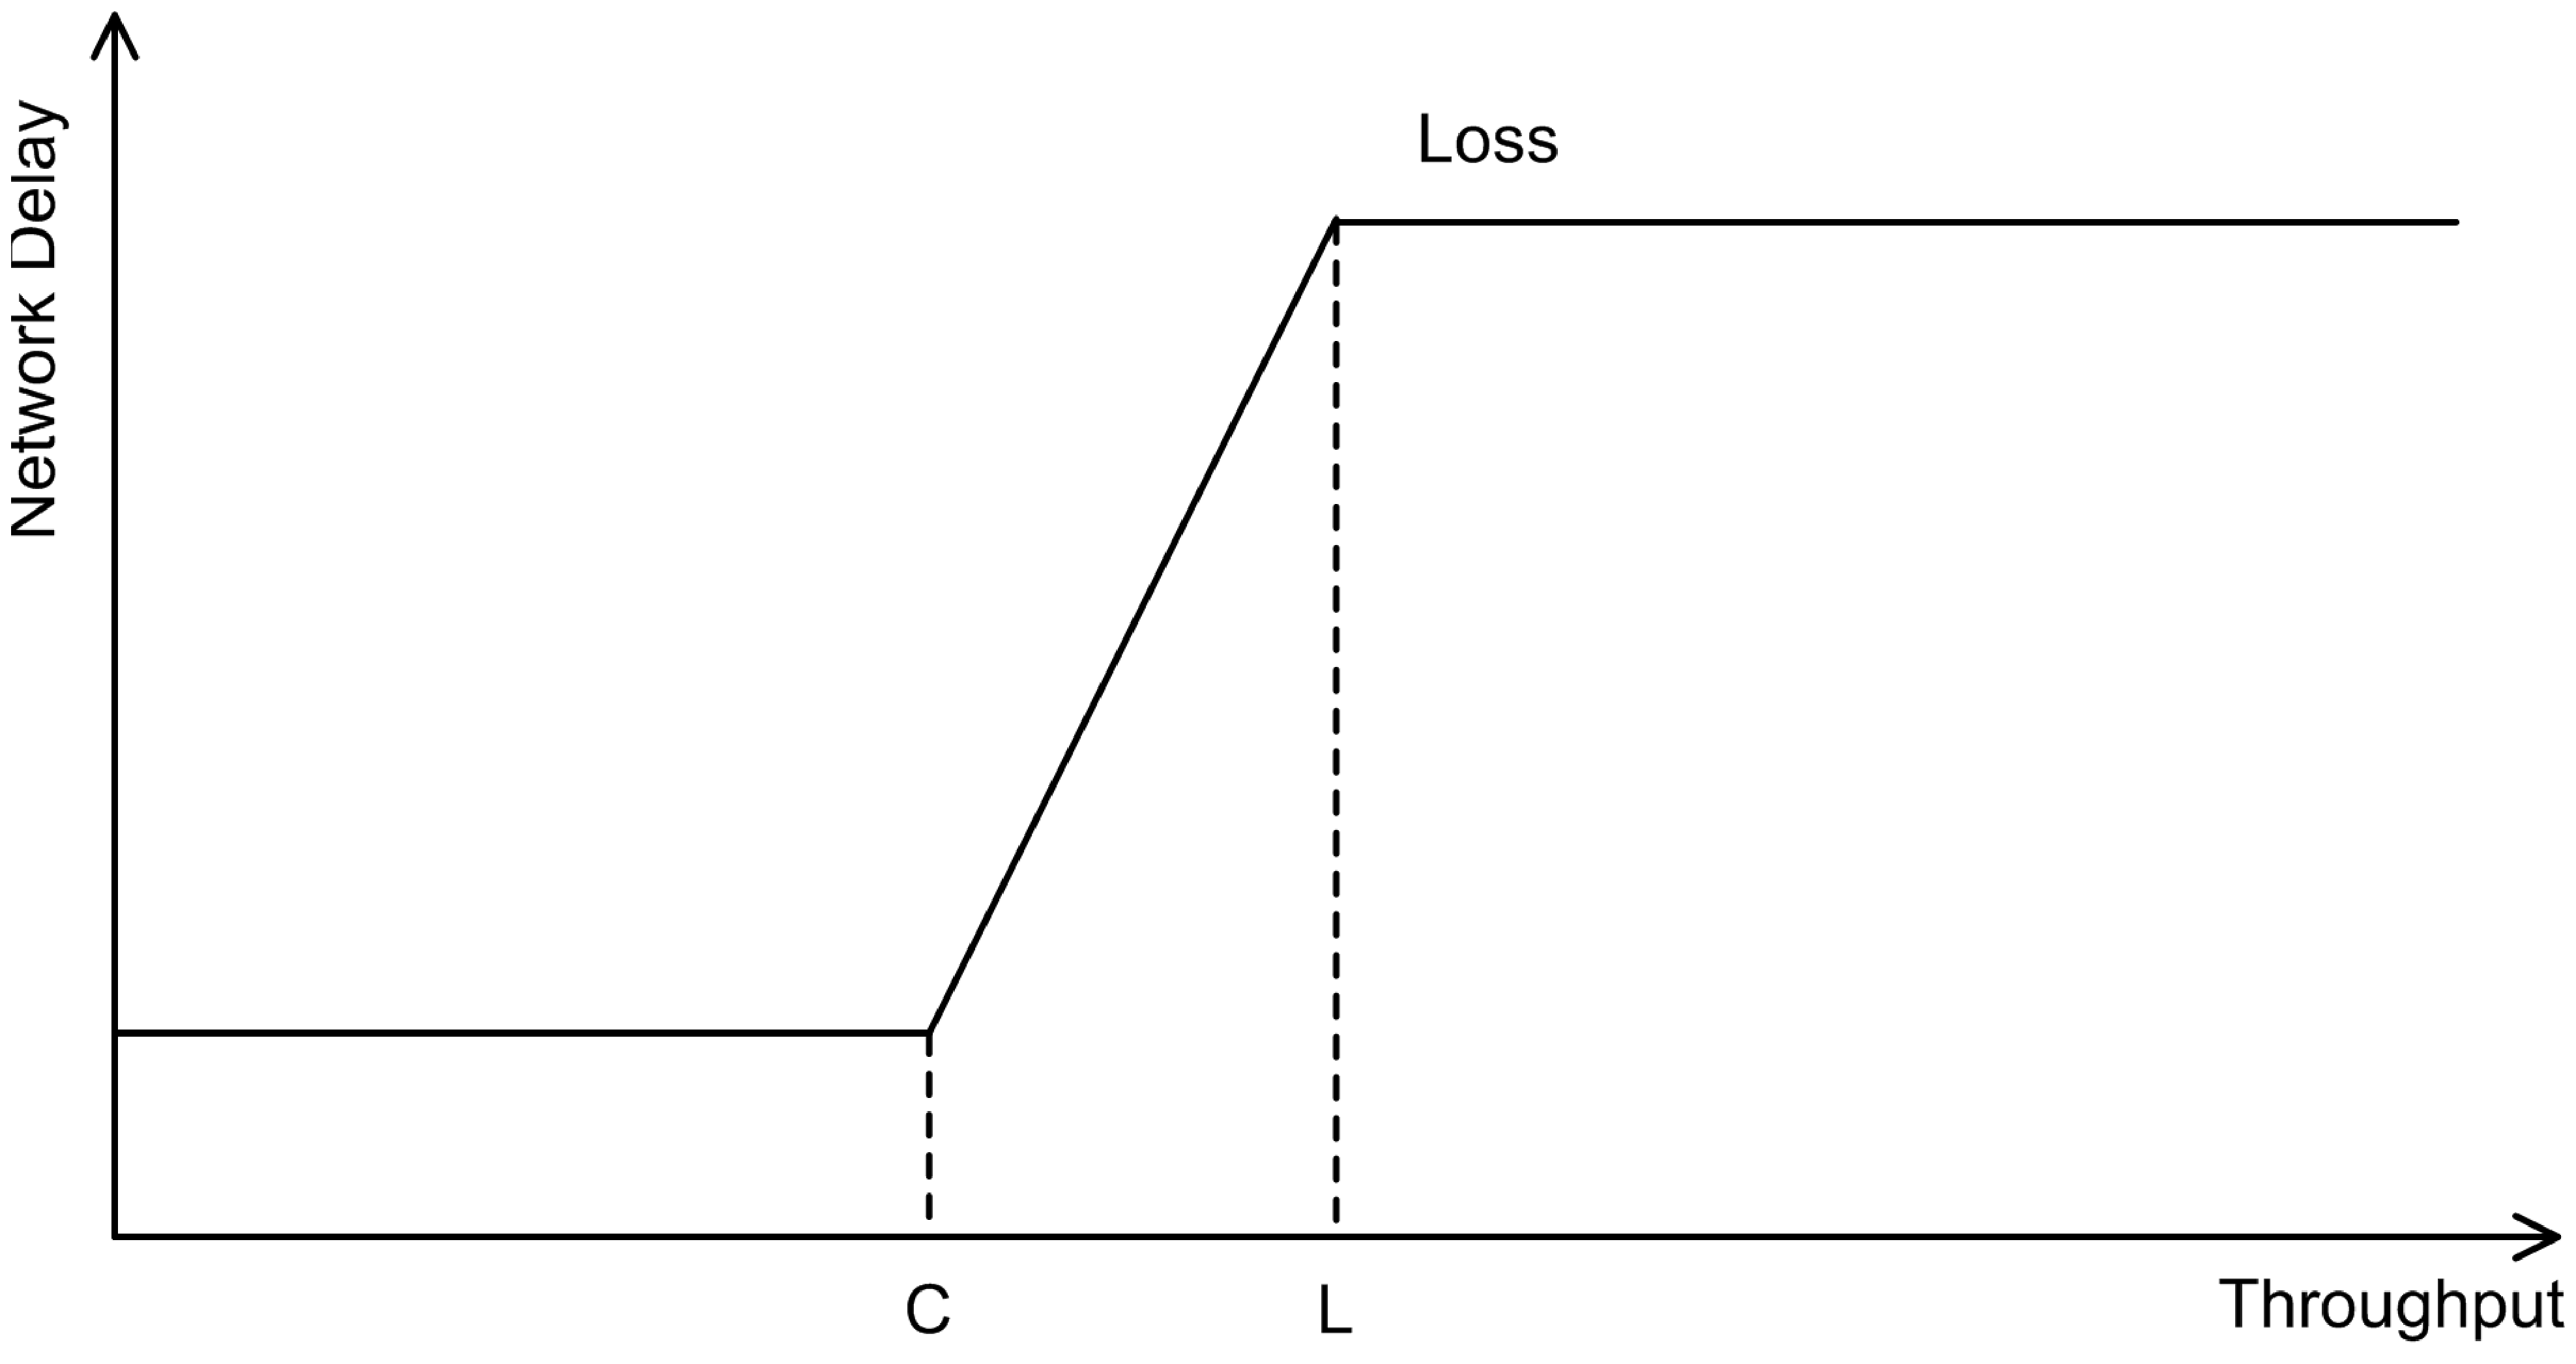
\includegraphics[width=0.8\linewidth]{fig/delay.eps}
\caption{Network delay trend as throughput increases}
\label{fig.delay}
\end{figure}

We can see that the queue on the path starts to accumulate at point $C$, but still, there is no loss. Starting from point $L$, the queue size overflows and packet loss happens. The minimum and maximum network delay for the path can be measured at point $C$ and point $L$. The difference between the real-time delay and minimum delay can be treated as the approximate queuing delay which represents congestion situation on that path. By observing the real-time queuing delay, we can adjust the weight of each path to properly assign future packets.

In Table~\ref{tb.pi}, except the column \emph{Real-Time Network Delay}, other three delay related columns are calculated through real time delay $D$.

\begin{enumerate}
\item \textbf{Minimum Network Delay $D_{min}$}. Every time one node receives update of network delay, it update this column with the minimum of its current value and the new real-time network delay.
\item \textbf{Real-Time Queuing Delay $Q$}. According to Figure~\ref{fig.delay}, the value of queuing delay is calculated as $Q=D-D_{min}$ which is the difference between real-time network delay and minimum network delay.
\item \textbf{Maximum Queuing Delay $Q_{max}$}. Maximum queuing delay is updated once the real-time queuing delay $Q$ is larger than $Q_{max}$. When packet loss happens, this value notates the curve section after point $L$ in Figure~\ref{fig.delay}.
\end{enumerate}


During our experiments, we found that calculating the weight of each path independently according to queuing delay can result in high fluctuation. So instead, we couple all the paths together and do micro adjustment to the weight of each path periodically as shown in Algorithm~\ref{alg.bw}.

\begin{algorithm}
\caption{Path Weight Incremental Adjustment.}
\label{alg.bw}
\begin{algorithmic}[1]
\STATE  $Q_{avg}= \frac{\sum_{i=1}^{N}Q_i}{N}$;
\IF {$Q_i\le Q_{avg}$}
    \STATE $W_i=W_i+S$;
    \IF {$W_i>1000$}
	    \STATE $W_i=1000$;
	\ENDIF
\ELSE
    \STATE $W_i=W_i-S$;
    \IF {$W_i<1$}
	    \STATE $W_i=1$;
	\ENDIF
\ENDIF
\STATE return;
\end{algorithmic}
\end{algorithm}

In Algorithm~\ref{alg.bw}, $N$ is the number of paths that belongs to one specific connection, $Q_i$ is the queuing delay of path $i$, $W_i$ is the path weight of path $i$, and $S$ is the adjustment granularity. Initially, every path has the same path weight of $\frac{1000}{N}$. In each loop, the path weight increases or decreases by $S$. The maximum value of the weight is $1000$. The minimum value is $1$ because we try to keep all the paths alive in case the congestion on a bad path has huge relief.

Algorithm~\ref{alg.bw} is executed periodically, the length of of period is defined as a configurable system variable $T$. So here, we have two configurable parameters which are the granularity $S$ and the period $T$. There is a trade-off here. Larger $S$ and shorter $T$ can generate higher fluctuation but faster convergence while smaller $S$ and longer $T$ can result in slow convergence and lower fluctuation. In our system, according to the path weight range ($1~1000$), we set $S$ to $10$ and $T$ to $100$ milliseconds. During our evaluation, this configuration can converge fast with low fluctuation.

\subsubsection{Customized Path Selection Framework}
\label{sec:resp}
In practice, maybe high throughput can represent most user requirements, but in some special cases, responsiveness can be of the first priority.

A typical example is Skype\cite{skype} calls. For Skype, audio packets and video packets are transmitted independently. In most scenarios, with responsive audio quality, real-time video streaming can be a bonus. But large delay in audio streaming can be a nightmare for a Skype call. In this case, obviously, audio packets and video packets have different priorities. During our study of Skype packets, although video packets can also be small, audio packets generally have substantially shorter length comparing to video packet. This provides a chance to define specific rules for Skype audio packets to achieve better user experience with lower delay.

Also, in a TCP connection with multipath, ACK packets are generally very small. On the other hand, delay in ACK packets can trigger TCP congestion control which results in unnecessary degradation of performance. By sending small ACK packets on the path with lower delay, unnecessary congestion control can be avoided, and further improve the overall performance of the connection.

To address the requirements above, we enable the users to define their own customized path selection policy based on the destination and length of packets. This customization provides a fundamental framework for more advanced path selection algorithms. A dedicated MPIP routing table is defined in Table~\ref{tb.route}.

\begin{table}[htbp]
\caption{\label{tb.route}MPIP routing table}
\centering
\begin{tabular}{|c|c|c|c|c|c|}
\hline
 IP   		&   Port   &          & Start  & End    & Routing       \\
 Address    &  Number     & Protocol & Size   & Size & Priority       \\
\hline
$*$&$23$&$TCP$&$0$&$200$&$P\_Res$   \\
\hline
$192.168.1.2$&$80$&$TCP$&$200$&$*$&$P\_Tp$   \\
\hline
$192.168.1.3$&$5221$&$UDP$&$0$&$500$&$P\_Res$  \\
\hline
\end{tabular}
\end{table}

When sending a packet, the system checks the destination IP address, port number, protocol and length of the target packet to get relative routing priority from Table~\ref{tb.route}. Different routing priority has different path selection policy. In our system, only two priorities are supported. $P\_Throughput$ means throughput is the first priority, the delay-based path selection algorithm in Section~\ref{sec:delay} will be used. When $P\_Response$ is referred, it means responsiveness is the first priority. In this scenario, the path that has the lowest delay will be chosen to send out the packet.

In the first row of Table~\ref{tb.route}, for any TCP connection with destination port $23$, if the packet length is smaller than $200$ bytes, the path with the lowest delay will be chosen, otherwise, delay-based algorithm is used. The second row actually is useless because all packets will use the delay-based algorithm even this row doesn't exist. The third row specifies that UDP packets sent to $192.168.1.3$'s $5001$ port will be assigned to the lowest delay path, otherwise, delay-based algorithm is used.

The same as regular routing table, the content of the MPIP routing table is configurable by users. In MPTCP, because all congestion control algorithms inherit from traditional TCP, it can't make the best of multipath. On the other hand, MPIP maintains paths in a more customized pattern, it is feasible to have application specific routing decisions. As we mentioned above, we only provide a basic framework for customized routing in MPIP. It only has limited functionalities. For example, it only specifies applications by port number. For some applications like P$2$P software, they have arbitrary port numbers, we can't locate the specific application in this case. There can also be other scenarios that our prototype doesn't work. But based on this framework, a more powerful and smarter routing decision mechanism can be completed.

%In Equation~\ref{eq.bw}, we update the path weight by progressive increasing to make the trend of path weight smooth. The increment consists of two parts. In the first part, we calculate the weight with the total network delay. For applications that prefer low delay to high throughput, assigning high priority to this part will be of much benefit. In the second part, we calculate the weight with queuing delay. This is beneficial for high bandwidth-delay product links according to \cite{mptcp}. By assigning high priority for this part, we can achieve high throughput.
%
%The parameter $C$ is used to adjust the weight of each part. For packets of different size, we have different calculation of $C$. For packets of small size, we can try more to send it out with a path with lower delay. On the other side, for packets of large size, we need to choose a path with less queuing delay which means lower congestion to send it out. To achieve this goal, the parameter $C$ is calculated through Equation~\ref{eq.c} where $L$ is the packet size and $MTU$ is the Maximum Transmission Unit of the NIC card. Applications like Skype have separate audio and video streaming, and users are more sensitive on audio delay. Generally voice packets have smaller length than video packets. According to Equation~\ref{eq.c}, when routing an audio packet, the delay-based routing calculation will get higher priority, and the packet will more likely be sent out through the interface that has low delay.
%
%
%$SI_q$ and $SI_d$ are the smooth index of queuing delay $Q$ and network delay $D$ of all paths calculated in Equation~\ref{eq.siq}  and Equation~\ref{eq.sid} where $N$ is the total number of paths in Table~\ref{tb.pi}. Please be noted that $Q_{max}$, $Q_{min}$ mean the maximum and minimum queuing delay out of all paths, while $D_{max}$, $D_{min}$ mean the maximum and minimum network delay in Equation~\ref{eq.bw}, Equation~\ref{eq.siq} and Equation~\ref{eq.sid}.
%%
%%\begin{eqnarray}
%%p'(4, 2, S_{4}) &=& \left. \frac{c_{c}(S_{4})}{4} + w(1 - \min(1, \frac{2}{12})2\rho(4))\right. \nonumber \\
%%&=& \left. \frac{c_{c}(S_{4})}{4} + w(1 - \frac{1}{3}\rho(4))\right. \label{schemeINotGroup4PeersPeer4}
%%\end{eqnarray}
%
%\begin{eqnarray}
%\label{eq.bw}
%W(k+1) = W(k) + \frac{C*D_{max}(k)}{\frac{D(k)-D_{min}(k)}{SI_d(k)}+1} \nonumber \\
%\left.		  + \frac{(100-C)*Q_{max}(k)}{\frac{Q(k)-Q_{min}(k)}{SI_q(k)}+1} \right.
%\end{eqnarray}
%
%\be
%\label{eq.sid}
%SI_d(k) = 100*(1-\frac{1}{N-1}\sum_{i=k-N+1}^{k-1}\frac{|D(i) - D(i-1)|}{D_{max}})
%\ee
%
%\be
%\label{eq.siq}
%SI_q(k) = 100*(1-\frac{1}{N-1}\sum_{i=k-N+1}^{k-1}\frac{|Q(i) - Q(i-1)|}{Q_{max}})
%\ee
%
%\be
%\label{eq.c}
%C = \frac{100 * L}{MTU}
%\ee
%
%Here we only explain the first part of Equation~\ref{eq.bw}, because the second part is almost the same.
%
%Given the path that has the minimum queuing delay $Q_{min}$, we calculate the difference of queuing delay of all paths with $Q_{min}$, and the path weight increases progressively with the inverse ratio of the difference. To avoid divide-by-zero error, factor $1$ is added to the difference.
%
%From Equation~\ref{eq.siq}, the calculated smooth index $SI_q$ is between $0$ and $100$, larger value of $SI_q$ means smoother queuing delay array which means that the current congestion status of each path is more similar, then it is safer to add larger weight value to each path. In the case of small $SI_q$, then congestion of each path has large variation, we need to take extra care to avoid fluctuations, so we reduce the added weight to each path.
%
%Because Linux kernel doesn't have good support of floating point calculation, $Q_{max}$ is set as the denominator to make sure denominator is larger than numerator to avoid zero increment. When the largest path weight in Tabel~\ref{tb.pi} hits a threshold value, all weight values will be normalized to the threshold value.
%
%For each path, when it is added into Table~\ref{tb.pi}, the same initial value will be assigned, after the system has achieved stability, each path will have a proper path weight value that reflects its capability.

%As shown in Figure~\ref{fig.weight}.
%
%\begin{figure}
%\centering
%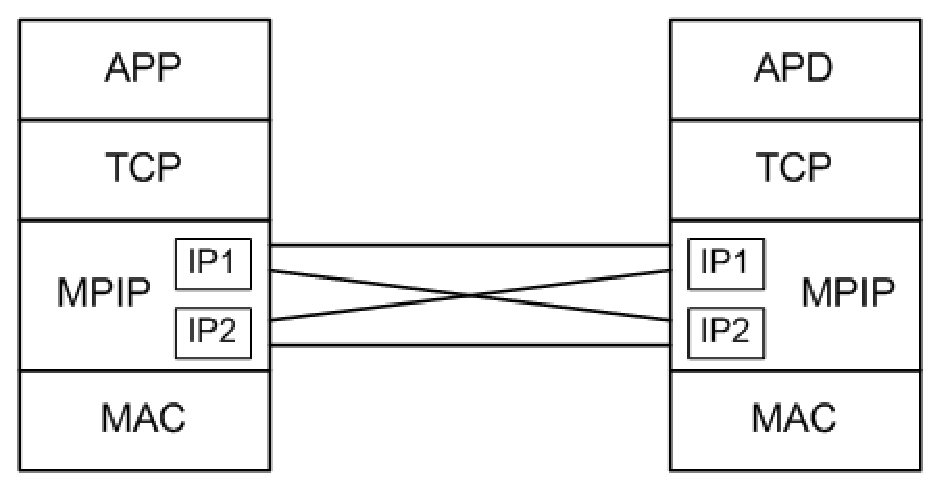
\includegraphics[width=1\linewidth]{fig/arch.eps}
%\caption{Path weight trend for each path}
%\label{fig.weight}
%\end{figure}

\subsection{Session Management}
\label{sec:session}

For one specific connection, it can be identified by a socket pair at each end. Each socket pair is described by a unique $4$-tuple consisting of source and destination IP addresses and port numbers. In our prototype, we call a connection's unique socket a session. To maintain all sessions, each MPIP enabled node maintains an instance of Table~\ref{tb.ss}.

\begin{table*}
\caption{\label{tb.ss}Session Information}
\centering
\begin{tabular}{|c|c|c|c|c|c|c|c|c|c|}
\hline
Node  & Session &  Source &  Source & Destination & Destination & Protocol  &    Next      & Update     \\
  ID  &   ID    &    IP   &   Port  &     IP      &    Port     &           &  Sequence No &  Time    \\
\hline
${ID}_1$&${SID}_1$&${SIP}_{1}$&${SPORT}_{1}$&${DIP}_{1}$&${DPORT}_{1}$&TCP&$S_1$&$T_1$               \\
\hline
${ID}_1$&${SID}_2$&${SIP}_{1}$&${SPORT}_{2}$&${DIP}_{1}$&${DPORT}_{2}$&UDP&$0$&$T_2$                 \\
\hline
${ID}_2$&${SID}_1$&${SIP}_{2}$&${SPORT}_{3}$&${DIP}_{2}$&${DPORT}_{3}$&TCP&$S_2$&$T_3$              \\
\hline
${ID}_2$&${SID}_2$&${SIP}_{2}$&${SPORT}_{4}$&${DIP}_{2}$&${DPORT}_{4}$&UDP&$0$&$T_4$                 \\
\hline
\end{tabular}
\end{table*}

For each connection, the system internally maintains a socket pair with source/destination IP addresses and port numbers, the system maintained socket information is the same as the pair maintained in Table~\ref{tb.ss}. The socket information for a session entry won't be modified after they have been added into Table~\ref{tb.ss} even the IP address that initiates the session doesn't exist any more. As will be shown later, the socket information in Table~\ref{tb.ss} is used to communicate with higher layer to guarantee seamless connection switching. If these information is modified, higher layers will notice the mismatch between the system maintained socket and MPIP maintained socket and causes connection failure.

\subsubsection{Addition/Removal of Sessions}

Session ID is the unique identity of one session. Unlike path ID in Table~\ref{tb.pi} which only requires to be unique locally, session ID needs to be unique on both ends of one connections which means that the session ID needs to be the same on both ends for the same session. But from Table~\ref{tb.ss}, we can see that different nodes can have the same session ID. Same as path ID, session ID is Arab numbers starting from $1$. This value is generated only when adding new sessions into Table~\ref{tb.ss}.

After the MPIP availability handshake has been successfully completed, when sending out a packet, the sender checks Table~\ref{tb.ss} to see whether a proper session entry has been generated. If not, one new record will be added. We extract the IP addresses, port numbers and protocol from packet headers, and gets the destination node ID from Table~\ref{tb.wi}, then it generates a new session ID and adds one new entry into Table~\ref{tb.ss}. After this, the new session ID will be filled into \emph{Session ID} in the CM block whenever packets are sent out on this connection. The receiver extracts the session ID and inserts one entry into its own Table~\ref{tb.ss}. This will make sure that for the same session, both sides of the connection have the same session id because only one side generates it.

Besides the session ID, all IP addresses and port numbers can be different in Tabel~\ref{tb.ss} of both sides because of NAT devices, this doesn't cause any problem because the IP addresses and port numbers only need to be the values that are seen locally.

Removal of sessions is decided by expiration. At each node, every time it sends or receives a non-heartbeat packet, it goes to Table~\ref{tb.ss} to get the session ID to fill the control message and updates the column \emph{Update Time}. For an active session, this time stamp should be updated frequently. If the timestamp expires a threshold value, the session is considered to be obsolete and removed from Table~\ref{tb.ss}. In our system, this threshold value is set to $120$ seconds. After all information related to this session is removed, if there are still more packets coming on that connection, MPIP handshake will start over.

Once session entry has been inserted into Table~\ref{tb.ss} at both side, different paths will be added into Table~\ref{tb.pi} and available to be chosen to transmit future packets that belong to this session according to path selection algorithms.

\subsubsection{NAT Consideration}

NAT devices can be the largest obstacle for MPIP. There are many types of NAT devices. Different type of NAT device does different modifications to Internet traffic. Generally, a NAT device changes the IP addresses and port numbers of a packet. But further, some application-level gateways can modify more content of a packet like the sequence numbers of TCP packets. We can still name many other different cases where NAT devices do customization to packets. In these scenarios, MPIP won't be able to perform correctly. Instead of designing an all-purpose MPIP system, we choose to fall back to regular connection in these case.

The value of the column \emph{Update Time} in Table~\ref{tb.ss} is also used to monitor the correctness of MPIP. As mentioned, this value is updated when packets are received on this session. In our system, if this value is not updated for $120$ seconds, this session is considered to be dead. But if this value is less than $120$ seconds and larger than $500$ms, we assume that MPIP is not working correctly, then this session falls back to regular connection and multipath feature is disabled. We set the value of $500$ms which is slightly larger than the period of heartbeat.

This mechanism works perfectly for connections that transmit packets with high intensity, e.g., chunky file download, video/audio streaming, etc. If for some reason the packets don't reach the destination at all through MPIP, the timer expires soon and falls back to regular connection. Specifically for TCP traffic, sometimes the packets reach the destination with modified header which the receiver can't recognize, the sending window of the connection becomes zero, traffic on both direction pauses soon, and finally the session falls back to regular connection.

But for applications that transmit packets intermittently, the connection may fall back to regular connection falsely. For example, a SSH session may idle for a long time because of no traffic at all. For these scenarios, we don't do any special process in our system, we just fall back as designed because if a connection is not active enough, the benefit it can get from MPIP is trivial.

Through this simple algorithm, we monitor MPIP's performance as a blackbox. MPIP can fail because of many factors on NAT issue, but no matter why MPIP is acting incorrectly, regular connection is always there to take over.


\subsubsection{Workflow of Sending/Receiving Packets}

For one regular packet, when being sent, it goes through application layer, transportation layer, then arrives at network layer where IP protocol resides in. Before the packet arrives at network layer, socket information inside the packet is the one that maintained by OS. In regular scenarios, the system finds a proper interface to push out the packet according to the destination IP address and routing table. The opposite flow is executed for inbound packets. For a MPIP enabled system, all the other operations remain the same except that of network layer.

For outbound packets, when the packet arrives at network layer from transportation layer, the system looks into Table~\ref{tb.ss}, and finds the session entry that matches socket information in the original packet, extracts the session ID to fill into field \emph{Session ID} in CM block. To choose the proper path to send out the packet, the first thing is to locate which paths in Table~\ref{tb.pi} are eligible for this connection. Given the destination IP address and port number in the socket information, we can find \emph{Node ID} in Table~\ref{tb.wi}, then in Table~\ref{tb.pi}, all entries that have the correct node ID and session ID are eligible. Among all these paths, the most suitable path will be chosen out through the mechanism introduced in Section~\ref{sec:path}.

The chosen path's path ID will be assigned to field \emph{Path ID} in CM block for delay measurement at the receiver, meantime, we modify the source and destination IP address/port number in the IP header and transportation layer header with the chosen path's source and destination IP address/port number. Then we route the packet with the new IP header information to a proper interface.

For inbound packets, when receiving a packet, the receiver extracts node ID and session ID in the CM block, with these two parameters, the receiver locates the original socket pair in Table~\ref{tb.ss}, and modify network layer header and transportation layer headers with source and destination IP address/port number from Table~\ref{tb.ss}. Fields related to path measurement will be processed as explained int Section~\ref{sec:path}. Now the packet is back to its original shape that can be recognized by higher layers, it is ready to be pushed up.


%The whole process of the sending and receiving packets is shown in Figure~\ref{fig.flow}.
%
%\begin{figure}
%\centering
%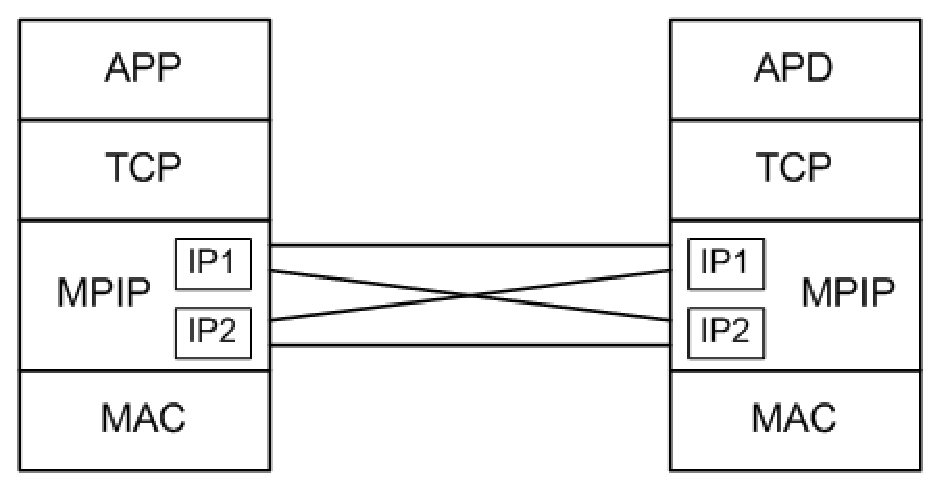
\includegraphics[width=1\linewidth]{fig/arch.eps}
%\caption{Work flow of sending and receiving a packet}
%\label{fig.flow}
%\end{figure}

\subsection{Multipath TCP Transmission}
\label{sec:tcp}
Through our experiments and previous studies\cite{mptcp}, NAT devices have a lot of interferences to end-to-end connections, especially for TCP packets. The most straightforward limitation for TCP packets is that many NAT devices will drop TCP packets that don't have a connection related to them. MPTCP doesn't have this problem because each subflow in MPTCP is a regular TCP connection. But in MPIP, if we transmit TCP packets on a path rather than the original one, NAT devices on the path will probably drop these packets before they arrive at the destination. To solve this problem, in our MPIP implementation, we provide two options to solve this problem.

\subsubsection{Fake TCP connection}
In NAT devices that drop TCP packets without relative connection information, we cheat them by constructing fake TCP connections. The construction of TCP contains three-way handshakes. Instead of constructing real TCP connections, we implement a simple three-way handshake at network layer which is similar as TCP handshake, but this connection information won't go up to TCP layer. All handshake packets have \emph{CM Flags} value of $Flags\_Hs$, these packets are dropped after being processed by MPIP.

As shown in Table~\ref{tb.cm}, the field \emph{Local Address List} carries all local IP addresses. Also, the node that initiates the connection is considered as the client. When the client receives the IP address list of the server, it extracts its own IP address list, then sends out a SYN packet through each possible path to the server except the original one which is the one that was used to initiate the connection. When the server receives this SYN packet, it replies with a SYN-ACK packet through the same path. After the client sends out the final ACK packet to the server, the three-way handshake for our fake TCP connection is completed successfully. After this, the path can be used to transmit TCP packets without being dropped.

In one specific TCP connection, we assume that the server has at least one public IP address for initiating the connection. But it is possible that other IP addresses on the server are not public, then the SYN packet will never arrive at that address, in this case, this interface will not be used at all.

\subsubsection{UDP wrapper}
The other option we provide for multipath TCP traffic is UDP wrapper. Because there is no connection information in an UDP packet, during our experiments, most NAT devices don't have any limitation on regular UDP traffic. We make use of this feature to wrap our TCP packet with a UDP header to pass the NAT devices and unwrap it when received.

At the sender side, every time the network layer gets a TCP packet from transport layer, the system chooses a path to send the packet out as shown in Section~\ref{sec:path}. If the chosen path isn't the original path, we wrap the user data and TCP header into an UDP packet. 

If UDP wrapper is used to transmit TCP traffic, when receiving one packet, we are capable to know this UDP packet is a wrapper for a TCP packet instead of a regular UDP packet by checking the column \emph{Protocol} in Table~\ref{tb.ss}. After removing the UDP wrapper, socket information will be extracted from Table~\ref{tb.ss} and filled into the TCP and IP header.

%\begin{figure}
%\centering
%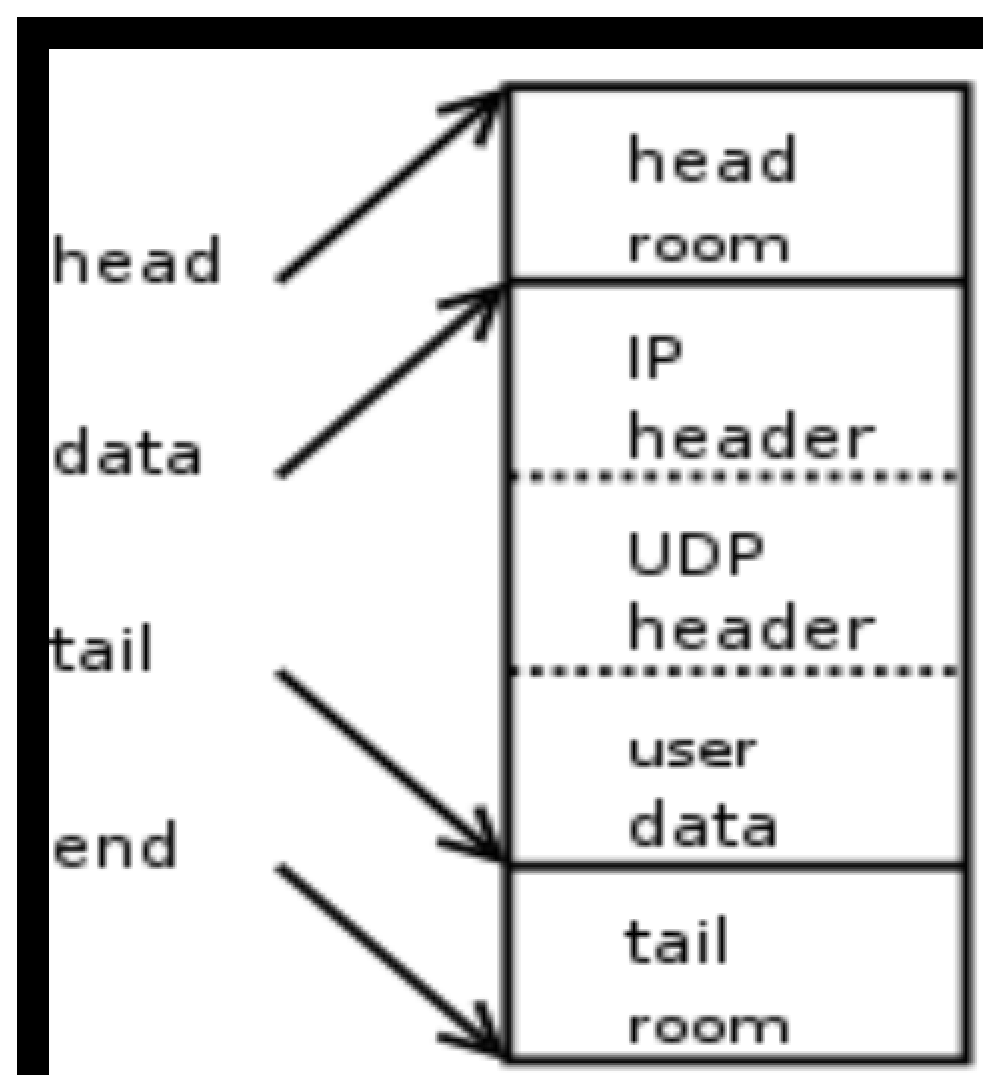
\includegraphics[width=0.8\linewidth]{fig/cm.eps}
%\caption{UDP wrapper for TCP packet}
%\label{fig.udpwrapper}
%\end{figure}

\subsubsection{Dealing with out of order TCP traffic}

In modern devices, different interfaces can have totally different delay behaviour. Generally, cellular interface has much larger delay than WiFi. For PC devices, wired connection generally has smaller delay than WiFi interface. Under this situation, packets can be out of order frequently during the life time of a connection. This is not a problem for protocols like UDP, but for TCP, as shown below, packet out-of-order can result in degradation of overall performance.

In TCP Congestion Avoidance algorithm, a retransmission timer expiring or the reception of duplicate ACKs can implicitly signal the sender that a network congestion situation is occurring. The sender immediately sets its transmission window to one half of the current size. When a duplicate ACK is received, the sender doesn't know if it is because a TCP packet was lost or simply that a packet was delayed and received out of order at the receiver. If the receiver can re-order TCP packet, it shouldn't be long before the receiver sends the latest expected acknowledgement. Typically no more than one or two duplicate ACKs should be received when simple out of order conditions exist. If however more than two duplicate ACKs are received by the sender, it is a strong indication that at least one packet has been lost, the sender does not even wait for a retransmission timer to expire before retransmitting the segment and enter control avoidance stage, the sender's transmission window is cut off by one-half. This is the fast retransmit algorithm.

%(the minimum of the congestion window and the receiver's advertised window size), but to at least two segments. If congestion was indicated by a timeout, the congestion window is reset to one segment, which automatically puts the sender into Slow Start mode. If congestion was indicated by duplicate ACKs, the Fast Retransmit and Fast Recovery algorithms are invoked.

Considering multipath scenario, if the delay behaviour difference among different paths is not trivial, we can expect a lot of out-of-order packets. This will result in many fast retransmit events, even TCP can go back to slow start stage. Given that in modern Internet, real packet loss has become rare event, most of transmission window cut-off events are unnecessary at all. In our prototype, to solve the heterogeneous delay performance of different paths, we make specific process of TCP out-of-order packets.

The overall process of out-of-order packet is shown in Figure~\ref{fig.outoforder}.

\begin{figure}
\centering
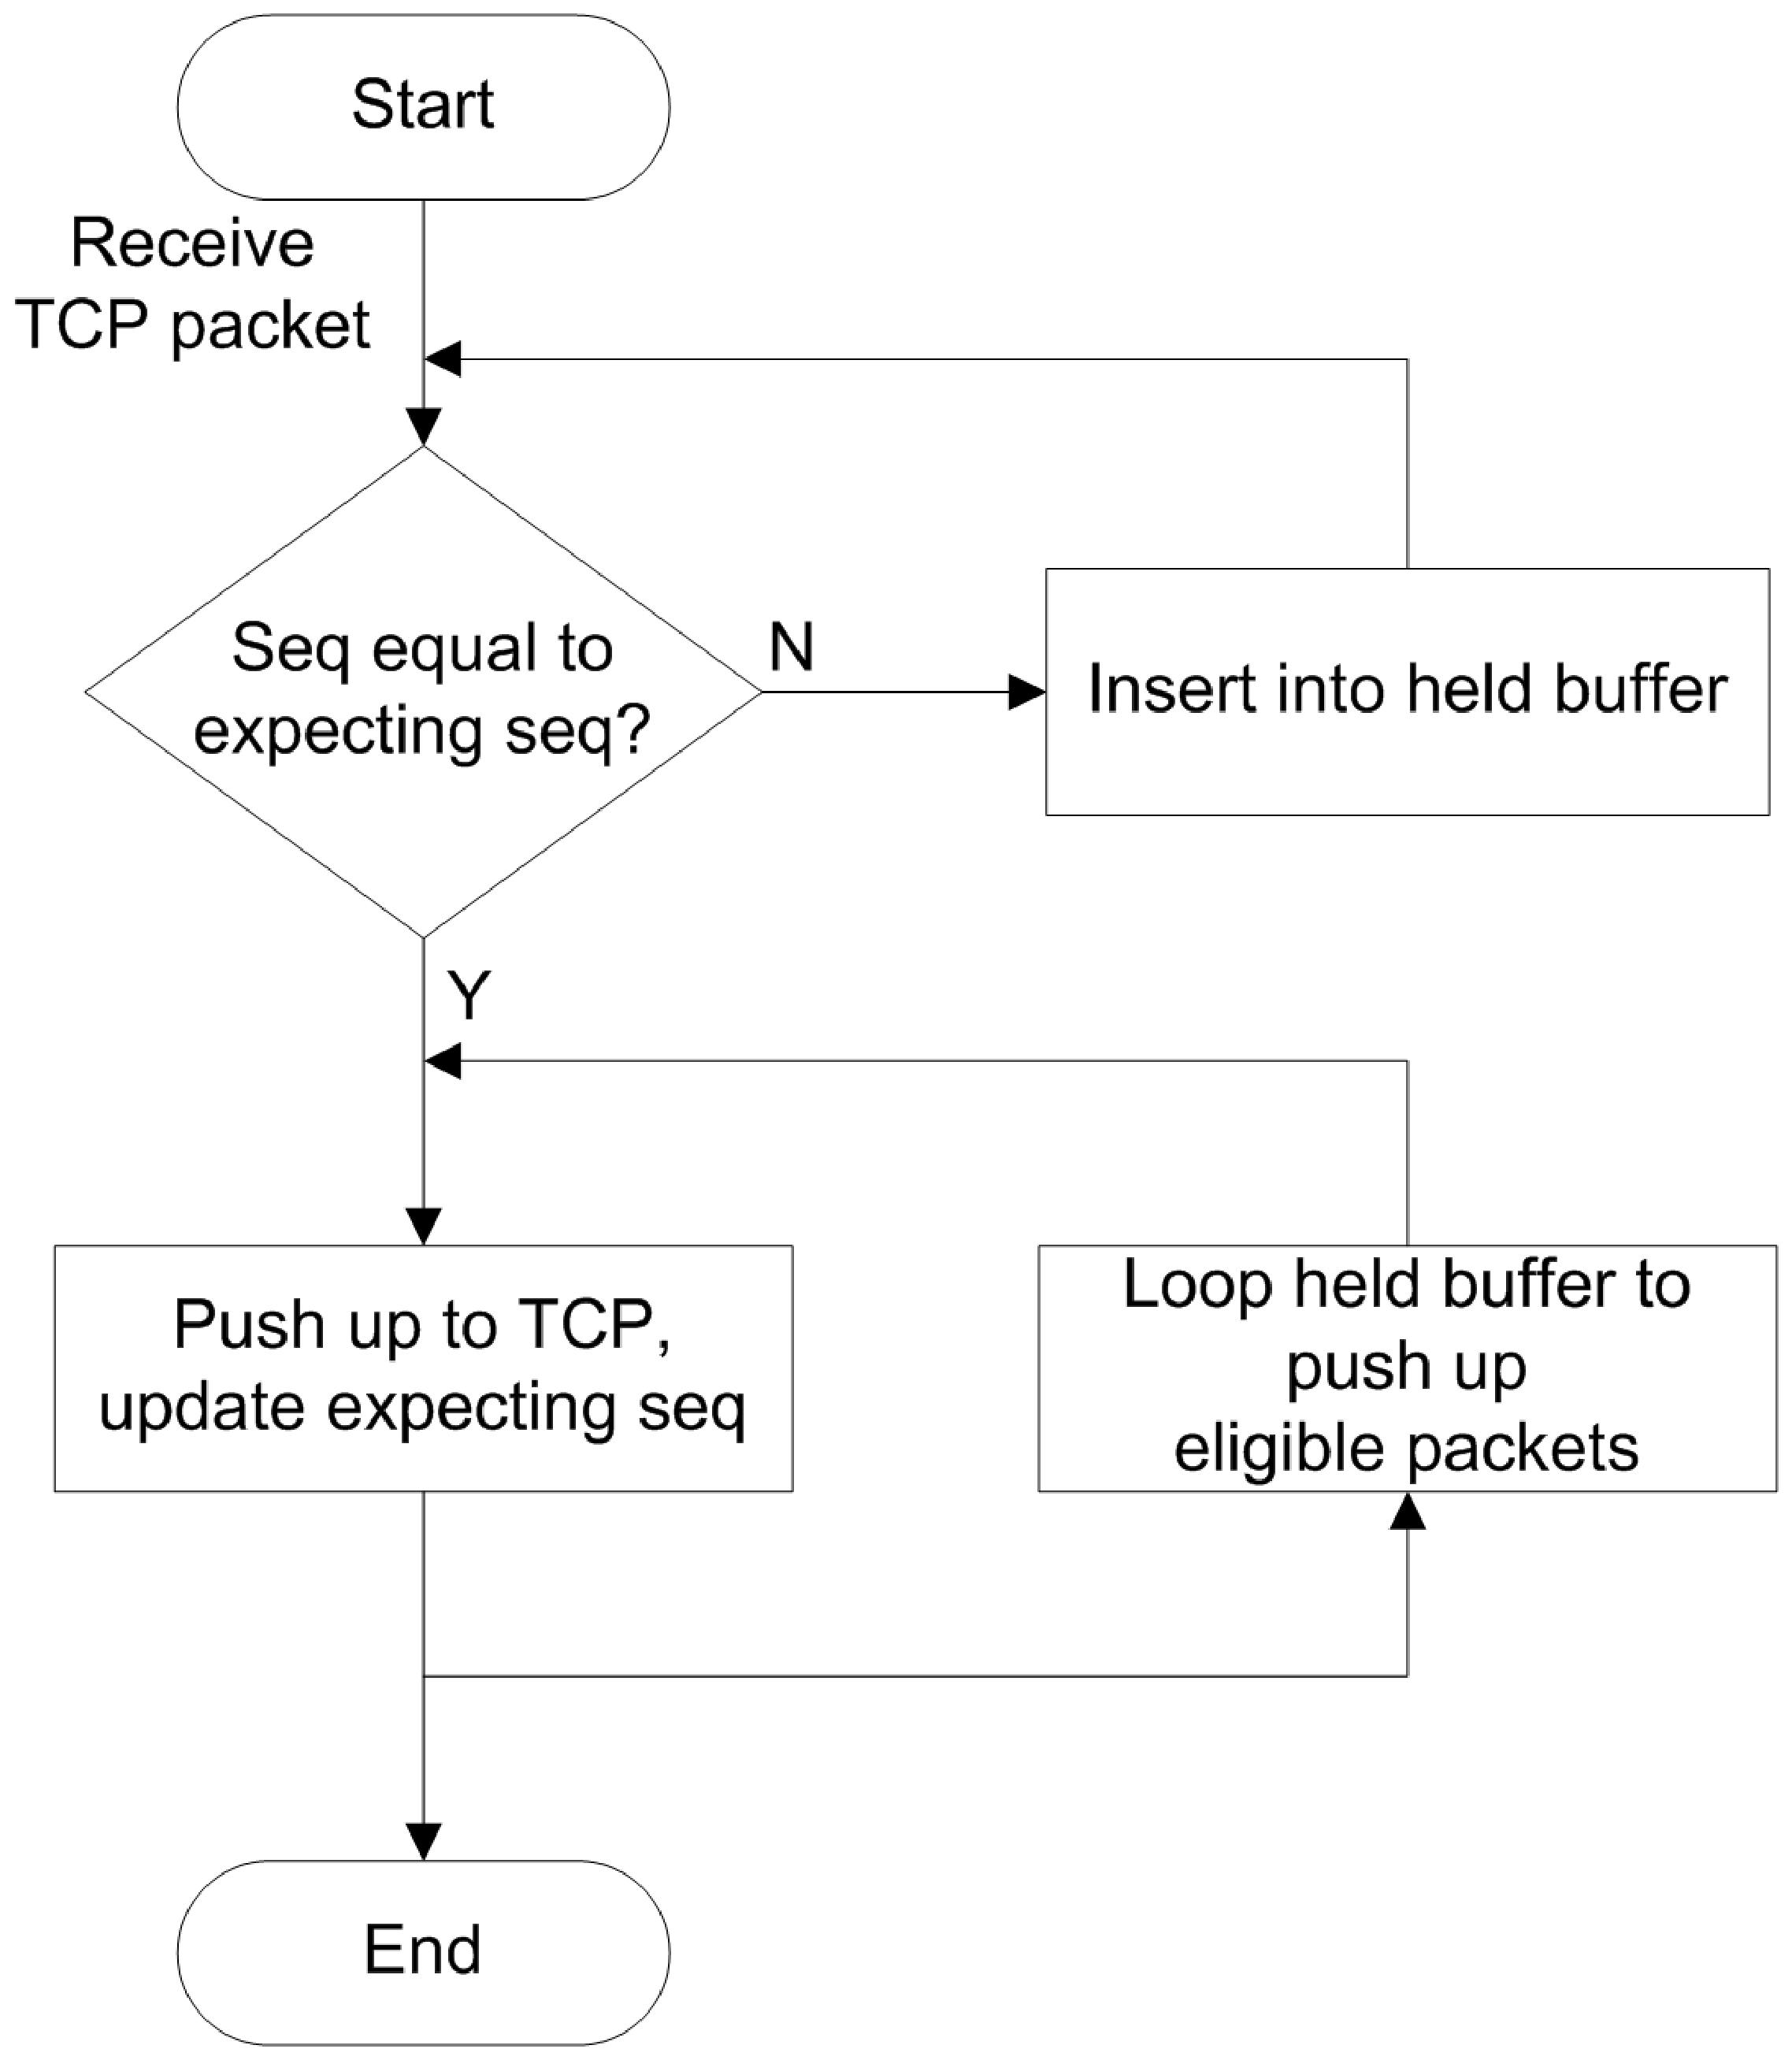
\includegraphics[width=0.8\linewidth]{fig/outoforder.eps}
\caption{TCP Out-Of-Order Packet Process}
\label{fig.outoforder}
\end{figure}


For each session in Table~\ref{tb.ss}, if it is TCP protocol, MPIP maintains a buffer $B$ to store all out-of-order packets and the next expecting sequence number $S$. Every time one node receives a TCP packet, it takes out the sequence number, if it equals with the current expecting sequence number of that session, the packet is pushed up to transportation layer immediately, also, the buffered packets will be checked to see whether there are qualified packet for delivery. If not, the packet will be buffered into $B$ for future delivery. Every time one packet is pushed up to transportation layer, the next expecting sequence number $S$ is updated through Equation~\ref{eq.seq} where $L$ is size of the whole packet, $H_{ip}$ is IP header size, and $H_{tcp}$ is TCP header size. TCP sequence number ranges from $0$ to $2^{32}-1$. Equation~\ref{eq.seq} can overflow $S$. But the data type of sequence number is unsigned integral, the number will loop back to $0$ automatically after that.

\be
\label{eq.seq}
S(k) = S(k-1)+(L-H_{ip}-H_{tcp})
\ee

For the data structure that holds the TCP packets, a proper choice is to implement it as a binary tree, but according to our observations, most out-of-order packets come in an incremental order, and they are held in the buffer because of one late packet, when that late packet arrives, all the held packets will be pushed up. For this reason, we simply implement this structure a sorted list, every out-of-order packet will be inserted into this list in ascending order according to the sequence number. The time complexity to insert this packet is almost $O(1)$ because most out-of-order packets arrive in an incremental order as mentioned.
When the expecting packet arrives, then all the waiting packets can be cleared from this list with a simple loop. This reduces code complexity greatly without sacrificing performance.

During our experiments, it happens that one specific packet can be late for a long time, like if the packet is lost. In this situation, holding all subsequent packets will halt the whole session because TCP layer will assume that all packets are lost, this will result in catastrophe for the connection. To address this problem, we set up the maximum size of the buffer. All the packets in the buffer will be forcefully pushed up once it is full. In our prototype, we set this maximum size to $10$.

\subsubsection{MPIP and MPTCP work together}
\label{sec:together}
As the first implementation of multipath, MPTCP gains huge attractions in research. During the development of our prototype, we try to do side-by-side comparison between MPTCP and MPIP when referring to TCP connection. Besides this, for investigation purpose, we merge them together to see how the system works.

Assume that there are $2$ NICs at each end, MPTCP will have $4$ subflows for the session while each subflow is an independent TCP connection. MPIP will have four paths for all these four subflows which means that there will be totally $16$ paths for one session in this case.

When MPIP and MPTCP combine together, if packet loss happens, MPIP will notice the high queuing delay of the dedicated path, and avoid assigning packets to that path by reducing the path weight to prevent the situation becoming worse, then subflows of MPTCP triggers TCP congestion control less than regular case. Adding with MPTCP's unique two-level sequence number mechanism, the load balancing among paths at MPIP enables MPTCP to make better use of each path and generate higher throughput. We will see how this combination works in Section~\ref{sec:evaluation}. 